

   

Given,
\begin{align}
    Y&=\sum_{r=1}^{n}a_rX_r
\end{align}
The characteristic function of a random variable Y is defined as
\begin{align}
    C_{Y}\brak{t}&=E[e^{itY}\\
    \implies C_{Y}\brak{t}&=E[e^{it\sum_{r=1}^{n}a_rX_r}]\\
    \implies C_{Y}\brak{t}&=\prod_{r=1}^{n}E[e^{ita_rX_r}]\\
    \implies C_{Y}\brak{t}&=\prod_{r=1}^{n}C_{X_r}\brak{a_rt}
\end{align}
By taking $a_r=2^{-r}$ we get,
\begin{align}
    C_{Y}\brak{t}&=\prod_{r=1}^{n}C_{X_r}\brak{\frac{t}{2^r}}
    \label{ma1997-8:a}
\end{align}
As random variables $X_r's$ follow discrete uniform distribution with only two possible outcomes ($X_r=-1$ and $X_r=1$) the characteristic equation of $X_r$ is
\begin{align}
    C_{X_r}\brak{t}&=\sum_{k}e^{ikt}\pr{X_r=k}\\
    \implies C_{X_r}\brak{t}&=\frac{e^{-it}}{2}+\frac{e^{it}}{2}\\
    \implies C_{X_r}\brak{t}&=\frac{1+e^{2it}}{2e^{it}}\\
    \implies C_{X_r}\brak{\frac{t}{2^r}}&=\frac{1+e^{2i\brak{\frac{t}{2^r}}}}{2e^{i\brak{\frac{t}{2^r}}}}
        \label{ma1997-8:b}
\end{align}
using \eqref{ma1997-8:b} in \eqref{ma1997-8:a}
\begin{align}
    C_{Y}\brak{t}&=\prod_{r=1}^{n}\brak{\frac{1+e^{2i\brak{\frac{t}{2^r}}}}{2e^{i\brak{\frac{t}{2^r}}}}}\\
    \implies C_{Y}\brak{t}&=\frac{\brak{1+e^{it}}\brak{1+e^{i\brak{\frac{t}{2}}}}....\brak{1+e^{i\brak{\frac{t}{2^{n-1}}}}}}{2^n\brak{e^{i\sum_{r=1}^n\frac{t}{2^r}}}}\\
     \therefore C_{Y}\brak{t}&=\frac{\brak{e^{2it}-1}}{2^ne^{it\brak{\frac{2^{n+1}-1}{2^{n+1}}}}\brak{e^{\brak{\frac{it}{2^{n-1}}}}-1}}
     \label{ma1997-8:c}
\end{align}
Now consider
\begin{align}
     \lim_{n\to\infty} C_{Y}\brak{t}
     \label{ma1997-8:d}
\end{align}
using \eqref{ma1997-8:c} in \eqref{ma1997-8:d}
\begin{align}
    \implies \lim_{n\to\infty}\frac{\brak{e^{2it}-1}}{2^ne^{it\brak{\frac{2^{n+1}-1}{2^{n+1}}}}\brak{e^{\brak{\frac{it}{2^{n-1}}}}-1}}
    \label{ma1997-8:e}
\end{align}
We know that,
\begin{align}
    \lim_{n\to\infty}\brak{e^{\brak{\frac{it}{2^{n-1}}}}-1} &= \frac{it}{2^{n-1}}
    \label{ma1997-8:f}\\
    \lim_{n\to\infty}e^{it\brak{\frac{2^{n+1}-1}{2^{n+1}}}}&=e^{it}
    \label{ma1997-8:g}
\end{align}
Using \eqref{ma1997-8:f} and \eqref{ma1997-8:g} in \eqref{ma1997-8:e}
\begin{align}
    \lim_{n\to\infty} C_{Y}\brak{t}&=\frac{\brak{e^{2it}-1}}{2ite^{it}}
%    \label{ma1997-8:h}
\end{align}
Now, let's assume that if $Y$ follows uniform distribution on (-1,1) then it's pdf can be written as
\begin{align}
    f_{Y}(y)=\begin{cases} 
            \frac{1}{2}  &  -1\le y\le 1\\
            0 &  otherwise
            \end{cases}
\end{align}
And it's cdf would be
\begin{align}
    F_{Y}(y)=\begin{cases} 
            0 & y<-1\\
            \frac{1+y}{2}  &  -1\le y\le 1\\
            1 &  otherwise
            \end{cases}
\end{align}
It's characteristic function would be 
\begin{align}
   C_{Y}\brak{t}&= \int_{-\infty}^{\infty} e^{ity}.f_{Y}(y) \,dy\\
    \implies C_{Y}\brak{t}&=\int_{-1}^{1} e^{ity}.\brak{\frac{1}{2}} \,dy\\
    \implies C_{Y}\brak{t}&=\frac{\brak{e^{2it}-1}}{2ite^{it}}
    \label{ma1997-8:h}
\end{align}
So from \eqref{ma1997-8:g} and \eqref{ma1997-8:h} we conclude that as $\brak{n\rightarrow\infty}$ $Y$ converges in distribution to uniform distribution on (-1,1).
\begin{figure}[h]
    \centering
    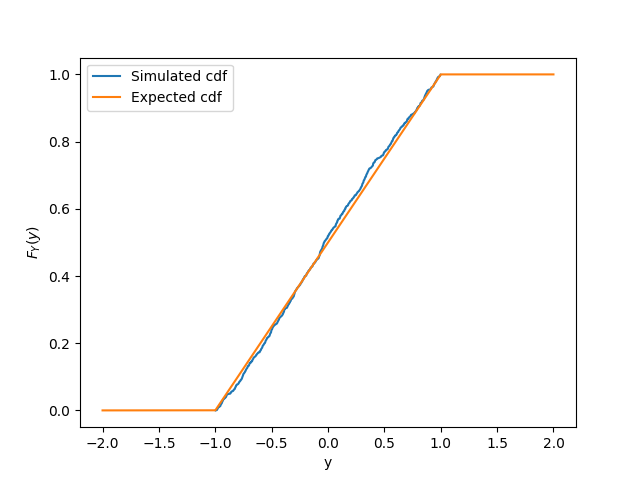
\includegraphics[width=\linewidth]{solutions/ma/1997/8/simulated_cdf.png}
    \caption{Simulated vs expected cdf plot of random variable Y}
    \label{ma1997-8:cdf_plot}
\end{figure}
